\documentclass[conference]{IEEEtran}
\usepackage{cite}
\usepackage{amsmath,amssymb,amsfonts}
\usepackage{algorithmic}
\usepackage{graphicx}
\usepackage{textcomp}
\usepackage{xcolor}
\usepackage{float}
\def\BibTeX{{\rm B\kern-.05em{\sc i\kern-.025em b}\kern-.08em
    T\kern-.1667em\lower.7ex\hbox{E}\kern-.125emX}}
\begin{document}

\title{Impulse Response Model for Switched Inductor Converters\\}

\author{\IEEEauthorblockN{Ryan J. Billing}
\IEEEauthorblockA{
\textit{Schweitzer Engineering Laboratories}\\
ryan\_billing@selinc.com}
\and
\IEEEauthorblockN{Alte R. Nate}
	\IEEEauthorblockA{
		\textit{Schweitzer Engineering Laboratories}\\
		alte\_rnate@selinc.com}
}


\maketitle

\begin{abstract}
Charging and discharging current waveforms are treated as an impulse response.
\end{abstract}


\section{Introduction}
Introduction TODO. 

\section{Background}

\subsection{Common Switched-Mode Converter Topologies Overview}

Boost, Buck-Boost, Flyback, Buck, Forward

\subsection{Switched-Mode Converters as Current Sources}

Detail how current sources can be inserted in-circuit representing currents during charging and discharging modes of each cycle.


\section{Dissection of the Sampled System}
Diagram the process of sampling, ZOH, resampling and impulse responses.



\section{Peak Current Control System}

Peak Current Mode Control is a technique used for controlling inductor currents in a switched-mode converter on a cycle-by-cycle decision-making interval. The control signal sets a threshold to limit inductor peak intake currents during the charging portion of the cycle. A compensating ramp is often added to the inductor's current sense signal to force pre-mature tripping of the comparator (the reason will become apparent later).

It is important to note that the peak current control signal is most commonly derived from the converter’s output voltage error amplifier, and this signal is not band-limited.

The difficulty with deterministic sampling of the control signal can be overcome by using an analytical technique which is compatible with the following assumptions:
\begin{enumerate}
	\item Steady-state and small signal behavior are of greatest interest.
	\item The large signal response can be characterized by evaluating small signal behavior over a range of steady-state operating points. 
	\item The peak current control threshold does not change during the sampling interval.
\end{enumerate}

The third assumption has material consequence to the high frequency dynamics of the model, but there is an analytical technique to handle this situation precisely.

The first observation is that the system being modeled is sampled at an instant in time when the sum of inductor peak current and compensation ramp exceed the comparator threshold. In the context of small signal analysis this sampler is periodic, and the sampling action can be expressed by multiplication of the peak current control signal with a Dirac comb function.

The frequency response of the sampler is flat up to half the switching frequency...

To   

 Fig.~\ref{cpm_waveforms} illustrates an analytical technique which can be used to enforce the validity of this assumption. 


\begin{figure}[ht]
	\centerline{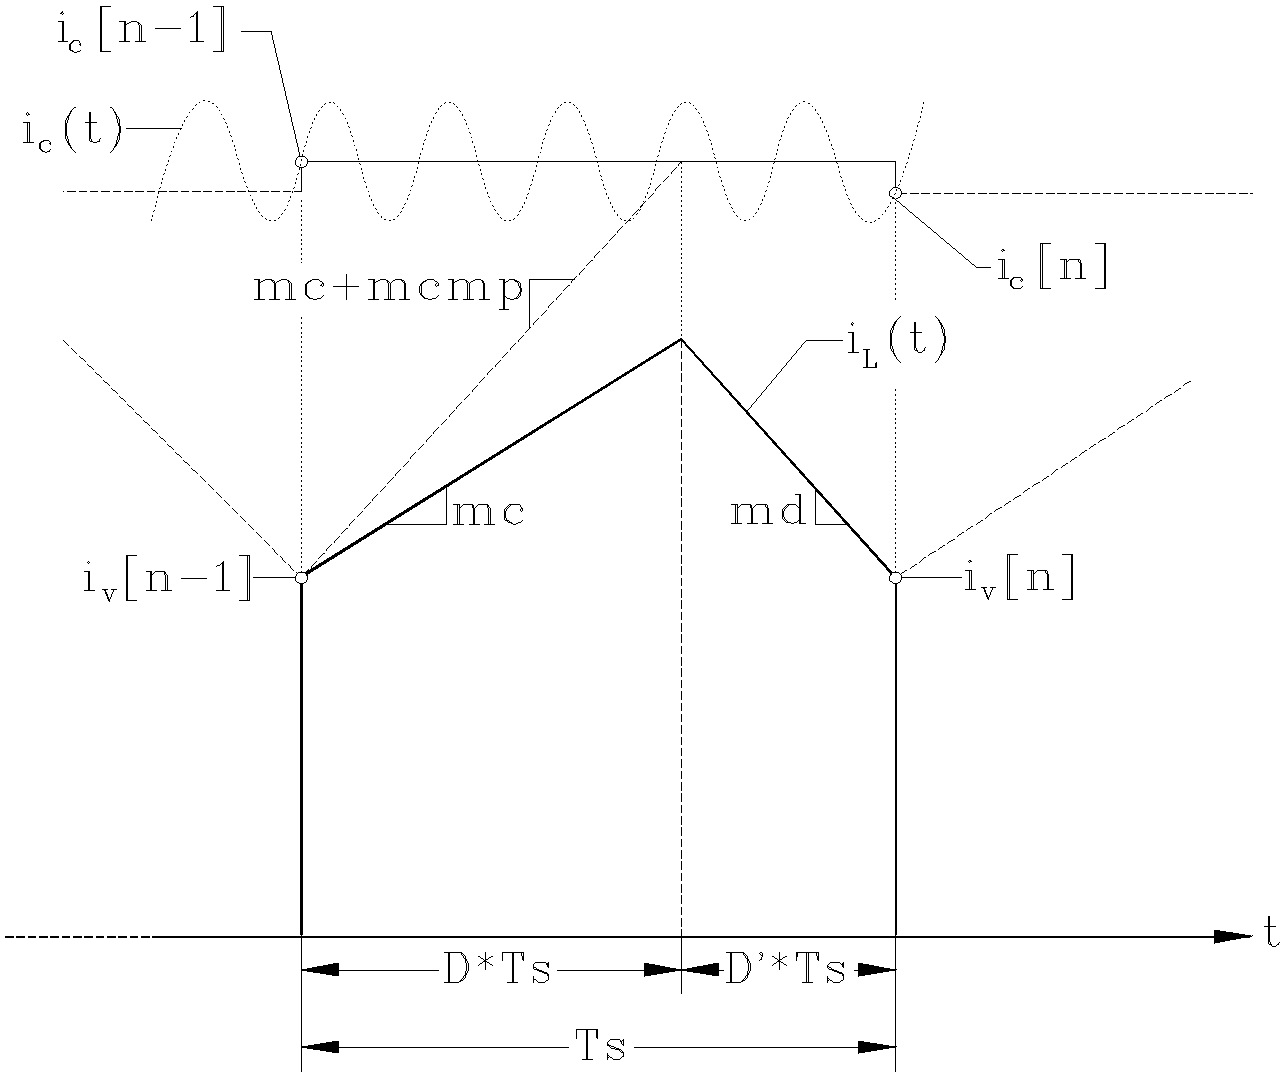
\includegraphics [
		width=7cm,
		keepaspectratio,
		] {a_cpm_waveforms.png}}
	\caption{Inductor waveforms with peak current mode control.}
	\label{cpm_waveforms}
\end{figure}

In \ref{cpm_waveforms} it has been made apparent that the control current  $ i_c[n]  $ is not band-limited.

\subsection{Derivation of the Discrete Time IIR Filter}
The analytical system presented in Fig.~\ref{cpm_waveforms} shows the peak current threshold being sampled synchronous to the valley currents and being held constant throughout the switching cycle.  If the charge, discharge and compensating slopes are also considered static throughout the sampling interval, then the system can be fully characterized on the rising edge of the primary gate drive signal (coincident with inductor valley currents).  The relationship between valley currents is then,
\begin{equation}
i_v[n] =  i_v[n-1] + m_c D T_{SW} - m_d  D' T_{SW}   \label{ivd}
\end{equation} 
\begin{align*}
\text{where, } \\
T_{SW} &= \text{Modulator switching (sampling) period} \\
D &= \text{Modulator duty cycle} \\
D' &= (1-D) \\
m_c &= \text{Slope of current during charge cycle (A/s)} \\
m_d &= \text{Slope of current during discharge cycle (A/s)}\\
i_v[n] &= \text{Inductor valley current.} \\
i_v[n-1] &= \text{Previous inductor valley current.} 
\end{align*}
The duty cycle can be re-expressed in the following terms,
\begin{equation}
D = \dfrac{i_c [n-1] - i_v [n-1]} {(m_c + m_{cmp})T_{SW}}
\end{equation}
\begin{align*}
\text{where, } \\
\alpha &= \frac{m_c + m_d} {m_c + m_{cmp}} \\
m_{cmp} &= \text{Slope compensation (A/s)}
\text{and time-varying signals,} \\
i_c[n] &= \text{Sampled peak current threshold.} 
\end{align*}
Then expanding $ D $ and $ D' $ in (\ref{ivd}), the following recurrence relation emerges,
\begin{equation}
i_v[n] =  \alpha i_c[n-1] + ( 1 - \alpha ) i_v [n-1] - T_{SW} m_d   \label{ivn}
\end{equation}

It is now apparent from (\ref{ivn}) the peak current controller has the form of a discrete-time IIR filter. If the assumptions used to build this difference equation result in negligible error, then the IIR filter is a Linear Time Invariant (LTI) system. Such a system can be evaluated using a conventional signals and systems approach for discrete-time functions.

\subsection{Z-transform of the Peak Current Controller}
Given a difference equation for an LTI system (as assumed in (\ref{ivn}) ) the z-transform can be evaluated by inspection.  
\begin{equation}
\mathcal{Z} \{ i_v[n] \} = I_v (z) =  \alpha I_c(z) z^{-1} + ( 1 - \alpha ) I_v (z) z^{-1}  \label{ivz}
\end{equation}
The resulting transfer function is then
\begin{equation}
H_v(z) = \frac {I_v(z)} {I_c(z)} = \frac {\alpha z^{-1}} {1 - (1-\alpha) z^{-1}}  \label{hvz}
\end{equation}
Eqn.~\ref{hvz} is correct if it can be shown that
\begin{equation}
 \mathcal{Z} \{ T_{SW} m_d \} = 0 \label{zconst}
\end{equation}
One way to dismiss the effect of the constant seen in (\ref{ivn}) is by use of the unit step response, time shift and time reversal properties of the z-transform.

The necessary relationships are included to maintain coherence in the approach being presented.

\begin{table}[H]
	\caption{Useful Z-transform Properties}
	\begin{center}
		\begin{tabular}{|c|c|c|}
			\hline
			\textbf{Description}& \textbf{Time Domain}& \textbf{Z-tranform}\\
			\hline
			Unit Step Response & 
			u[n] =
			$ \begin{cases} 
				0 & n < 0 \\
				1 & n \geq 0 
			\end{cases} $ 
			 & U($ \mathit{z} $) = $\dfrac{1}{1-z^{-1}}$ \\
			\hline
			
			
			Time Reversal& u[-n]& U($ \mathit{z^{-1}} $) = $\dfrac{-z^{-1}}{1-z^{-1}}$  \\
			\hline
			Unit Delay & u[n-1] & U($ \mathit{z^{-1}} $) = $\dfrac{z^{-1}}{1-z^{-1}}$  \\
			\hline

		\end{tabular}
		\label{tabun}
	\end{center}
\end{table}

The choice of relationships expressed in Table \ref{tabun} plays on the following time-domain property. 
\begin{equation}
u[n-1] + u[-n] = 1 \label{funny_one}
\end{equation}
Any constant can be multiplied by one, which may be expanded according to (\ref{funny_one}), and then the z-transform becomes straightforward. Specifically when the constant is $ k = -T_{SW} m_d $,
\begin{equation}
	\mathcal{Z}\{ k * 1 \} = 
	\mathcal{Z}\{ k (u[n-1] + u[-n]) \}
\end{equation}
hence,
\begin{equation}
\mathcal{Z}\{ k \} = k \bigg( \dfrac{z^{-1}}{1-z^{-1}} + \dfrac{-z^{-1}}{1-z^{-1}} \bigg) = 0
\end{equation}


\subsection{Peak Current Controller Stability Analysis}

The expression in (\ref{hvz}) becomes unstable in the cases when the denominator approaches zero. Using Euler's formula, the complex exponential term in the denominator expands to the following.
\begin{equation}
	z^{-1} = e^{-j \omega T_{SW}} = \cos (\omega T_{SW}) - j \sin (\omega T_{SW}) 
\end{equation} 
The only condition in which the denominator can go to zero is $\omega T_{SW} = \pi$, when the imaginary part goes to zero.

In that case, $e^{-j \pi} = \cos ( \pi) = -1$, and the transfer function becomes
\begin{equation}
H_V(z) |_{\dfrac{\omega_{SW}}{2}} = \dfrac{\alpha (-1)}{1 - (1 - \alpha) (-1)} = \dfrac{- \alpha}{2 - \alpha} \label{cpmstability}
\end{equation}
The condition for stability therefore requires that $\alpha \le 2$.  The system is outside of the Region of Convergence (ROC) for $\alpha > 2$. It is intuitive from the time-domain expression in (\ref{ivn}) that any condition for which the magnitude of $(1 - \alpha)$ equals or exceeds 1.0, the state variable $i_v[n]$ will build rather than decay.
Recall that $\alpha$ is a function of inductor current slopes as well as the ramp compensation parameter, $m_{cmp}$.  It then follows from (\ref{cpmstability}) that the minimum amount of slope compensation required for stability is
\begin{equation}
m_{cmp} > \dfrac{m_d - m_c}{2} \label{slope_stab}
\end{equation}

\subsection{Comparison to Conventional Approach}
In $[ref]$ Middlebrook, Tan state the condition for stability in the peak current controller per following.

\begin{equation}
D'_{min} = \dfrac{0.5}{1 + \dfrac{m_{cmp}}{m_{mc}}} \label{transl_stab}
\end{equation}

The expression in (\ref{transl_stab}) makes use of notation consistent with the current text.

The steady-state condition within the peak current mode controller occurs when $i_v[n] - i_v[n-1]$. Evaluation of (\ref{ivd}) in the steady state condition yields the following.
\begin{equation}
	D T_s{SW} m_c - D' T_{SW} m_d = 0 \label{dsteadystate}
\end{equation}

Substituting $D' = (1-D)$, the expression in (\ref{dsteadystate}) is manipulated into the following form.
\begin{equation}
	D' = \dfrac{m_c}{m_c+m_d} \label{dp_mc_md}
\end{equation}
Combining (\ref{transl_stab}) and (\ref{dp_mc_md}),
\begin{equation}
	\dfrac{m_c}{m_c + m_d} = \dfrac{0.5}{1 + \dfrac{m_{mcmp}}{m_c}} \label{tan_stab_eq}
\end{equation}
Then solving (\ref{tan_stab_eq}) for slope compensation yields the following.
\begin{equation}
	m_{mcmp} = \dfrac{m_d - m_c}{2} \label{mid_stab}
\end{equation}

The inequality expressed in (\ref{slope_stab}) is obtained from (\ref{mid_stab}) when $D'$ in (\ref{dp_mc_md}) is evaluated in the limit as $D'$ approaches $D'_{min}$.

\subsection{Peak Current Controller Peaking}
Peak controller expression for peaking.

\section{Average Currents FIR Filters}
Derive expression or FIR filters for charging and discharging currents.

\subsection{Small-Signal Analysis}

\subsubsection{Discharging Current Small-Signal Behavior}

\subsubsection{Charging Current Small-Signal Behavior}

\subsection{Impulse Response Analysis}
\subsubsection{Frequency Response of Discharging Current}
\subsubsection{Frequency Response of Charging Current}
Example inline citation
\cite{b6}.

\begin{thebibliography}{00}
\bibitem{b1} G. Eason, B. Noble, and I. N. Sneddon, ``On certain integrals of Lipschitz-Hankel type involving products of Bessel functions,'' Phil. Trans. Roy. Soc. London, vol. A247, pp. 529--551, April 1955.
\bibitem{b2} J. Clerk Maxwell, A Treatise on Electricity and Magnetism, 3rd ed., vol. 2. Oxford: Clarendon, 1892, pp.68--73.
\bibitem{b3} I. S. Jacobs and C. P. Bean, ``Fine particles, thin films and exchange anisotropy,'' in Magnetism, vol. III, G. T. Rado and H. Suhl, Eds. New York: Academic, 1963, pp. 271--350.
\bibitem{b4} K. Elissa, ``Title of paper if known,'' unpublished.
\bibitem{b5} R. Nicole, ``Title of paper with only first word capitalized,'' J. Name Stand. Abbrev., in press.
\bibitem{b6} Y. Yorozu, M. Hirano, K. Oka, and Y. Tagawa, ``Electron spectroscopy studies on magneto-optical media and plastic substrate interface,'' IEEE Transl. J. Magn. Japan, vol. 2, pp. 740--741, August 1987 [Digests 9th Annual Conf. Magnetics Japan, p. 301, 1982].
\bibitem{b7} M. Young, The Technical Writer's Handbook. Mill Valley, CA: University Science, 1989.
\end{thebibliography}


\end{document}
